\chapter{Design}
\renewcommand{\kapitelautor}{Autor: Niklas Kienreich}

\section{Hintergedanken}
Genau, wie bei allen anderen Aspekten, dieser Diplomarbeit, war der Hintergedanke des Designs, es einladend, fröhlich und angemessen der Zielgruppe zu gestalten.

\section{Corporate Design}
Bei einem Corporate Design handelt es sich um die Summe aller grafischen, beziehungsweise visuellen Informationen eines Unternehmens. Ein solches Corporate Design birgt einige Vorteile.
Ein Vorteil wäre zum Beispiel die Kontinuität der Unternehmenskommunikation. Dadurch wird Vertrauen aufgebaut und gefördert. Außerdem erhöht es durch eben jene Kontinuität die Bekanntheit des Unternehmens und kann auch Kosten sparen. \footnote{\label{} vgl.https://www.beinert.net/corporate-design/ [Zugriff: 01.04.2018]}
\subsection{Farben}
Hier musste, wie bei den Hintergedanken schon erklärt, an die Zielgruppe gedacht werden. Zum Beispiel haben Männer und Frauen unterschiedliche Präferenzen bei Farben. Diese können sich im Laufe, der Zeit sogar ändern. Anfangs des 20. Jahrhunderts, war Pink eine Farbe, die von Männern bevorzugt wurde, während Frauen sich Blau verbundener fühlten.\footnote{\label{} vgl.http://www.farbenlehre.com/grundlagen-der-farbenlehre/farbpraeferenzen-geschlecht [Zugriff: 02.04.2018]} Also ist die Farbwahl garnicht so einfach, wie man denken mag. Bei den Farben für Insight, wurde zum einen, ein helles Grün, zum anderen ein knalliges Orange gewählt. Als Akzentfarbe wurde ein helles Grau in das Corporate Design aufgenommen.

\begin{figure}[H] 
  \centering
     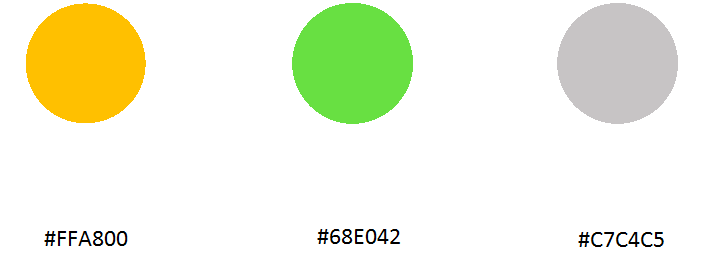
\includegraphics[width=0.7\textwidth]{design_abb1.png}
  \caption{Drei Farben des Corporate Design}
\end{figure}

\subsubsection{Grün}
Wenn etwas ergrünt, ergibt sich Hoffnung auf neues Leben. Diese Farbe ist sehr naturbelassen und die Farbpsychologie lehrt, dass Grün Lebensfreude und Jugend vermittelt. Grün kann zwar auch Gift und somit eine Warnung signalisieren, durch den Kontext der Webseite ist dies aber unwahrscheinlich. \footnote{\label{} vgl.http://www.grafixerin.com/bilder/Farbpsychologie.pdf [Zugriff: 17.03.2018]}

\subsubsection{Orange}
Bei Orange handelt es sich um eine sehr auffällige Farbe. Sie ist eine warme, energiegeladene Farbe und kann aufregend, bis sogar spaßig auf einen Menschen wirken. Durch ihre Auffälligkeit kann sie aufdringlich oder extrovertiert wirken. Orange kann auch billig wirken, da der Mensch kaum etwas Hochwertiges kennt, dass diese Farbe besitzt. \footnote{\label{} vgl.http://www.grafixerin.com/bilder/Farbpsychologie.pdf [Zugriff: 17.03.2018]}

\subsection{Typografie}
\subsubsection{Parisien Night Oblique}
Diese Schrift wurde wegen ihrer dynamischen Linienführung gewählt, welche an das Logo erinnert. Es sollte eine verspielte Abwechslung zu den Texten mit Calibri bieten. Die Schrift sieht fast so aus, als wäre sie mit freier Hand geschrieben worden, was eine Verbindung zu der Kreativität, in der Medientechnik bringen soll.
\\
Verwendung findet die Schrift in den Überschriften der Website.

\subsubsection{Calibri}
Calibri ist eine serifenlose Schrift. Sie ist dadurch auf Bildschirmen mit geringerer Auflösung leicht zu lesen. Sie wirkt durch ihre abgerundeten Ecken freundlicher, als manch andere Schriftart.\footnote{\label{} vgl.https://www.typografie.info/3/Schriften/fonts.html/calibri-r61/ [Zugriff: 18.03.2018]} Die Kombination aus Freundlichkeit und einfacher Lesbarkeit, war ausschlaggebend für die Wahl, dieser Schrift. Die Freundlichkeit ist ein selbstverständlicher Faktor, der auf der Website vermittelt werden soll, aber natürlich soll auch verhindert werden, dass der Leser beim Lesen der Texte überansprucht wird.
\\
Calibri wird in den Texten der Website und in den Textslides der Videos verwendet.

\subsection{Adobe Illustrator}
Der Adobe Illustrator ist ein ein Programm zum erstellen und bearbeiten von Vektorgrafiken. Er wird großteils für die Erstellung von Logos, Symbolen, Skizzen und sogar typografischen Elementen genutzt.\footnote{\label{} vgl.https://www.adobe.com/at/products/illustrator.html?sdid=V6NZKW2K\&mv=search\&s\_kwcid=AL!3085!3!247433680443!b!!g!!adobe\%20illustrator\&ef\_id=WhhSTwAAAD0HOQZA:20180401113957:s [Zugriff: 01.04.2018]}
\subsubsection{Vektorgrafiken}
Vektorgrafiken kann man beliebig vergrößern und verkleinern, ohne dass sie an Auflösung, Qualität oder allgemein Daten verlieren. Das liegt daran, dass Vektorgrafiken aus Linien und Kurven bestehen. Diese zusammen bilden sogenannte Pfade. Was diese Pfade so speziell macht und die verlustfreie Skalierung ermöglicht, ist dass sie durch mathematische Funktionen beschrieben werden. Das heißt, dass das Bild auf jeder erdenklichen Größe neu berechnet und gerendert werden kann. Das macht Vektorgrafiken für den Printbereich so interessant. Egal ob sich ein Logo auf einer kleinen Visitenkarte, oder auf einer riesigen Plakatwand befindet, es ist immer gestochen scharf. Sowohl das Logo und die Visitenkarte von Insight, als auch mehrere Grafiken auf der Website, wurden als Verktorgrafiken erstellt.
\footnote{\label{} vgl.https://helpx.adobe.com/illustrator/using/drawing-basics.html [Zugriff: 18.03.2018]}\footnote{\label{} vgl.http://www.vektorgarten.de/vektor-grafik-anwendung.html [Zugriff: 01.04.2018]}

\subsection{Logo}
\subsubsection{Logo-Arten}
Bei Logos unterscheidet man zwischen vier verschiedenen Arten. \footnote{\label{} vgl.http://www.webmasterpro.de/design/article/logodesign-arten-von-logos.html [Zugriff: 18.03.2018]} \footnote{\label{} vgl.http://www.sanseg.de/logodesign/zeichenmarken/ [Zugriff: 18.03.2018]}
\\
\\
Zum einen gibt es sogenannte Bildmarken. Hierbei handelt es sich um eine einfache Abbildung oder Illustration. Empfehlenswert ist solch ein Logo jedoch eher für größere Firmen und Unternehmen, da der Betrachter beim Erblicken des Logos, die Verbindung mit jenem Unternehmen herstellen können soll. Dies ist bei unbekannten Marken unwahrscheinlich und somit kontraproduktiv. Wenn ein Unternehmen auf eine Bildmarke umsteigt, gibt es oft eine Einführungsphase, in der das neue Logo anfangs mit Beschriftung gezeigt wird.
\\
\\
Eine weitere Logo-Art ist die Wortmarke. Sie zeigt einfach den Namen, des Unternehmens. Aber auch hier muss man sich Gedanken machen, wie das Logo auf den Betrachter wirkt. Neben der Farbe des Schriftzugs, sind typografische Aspekte auch wichtig. Darauf wird später in der Umsetzung des Logos genauer eingegangen.
\\
\\
Zeichenmarken sind den Wortmarken sehr ähnlich, denn sie beruhen auch auf der Typografie. Der Unterschied liegt darin, dass es sich hier nicht um Worte im Logo handelt, sondern um Abkürzungen, einzelne Buchstaben oder Zahlen.
\\
\\
Bei Wort-Bild-Marken, oder auch Kombinationen, handelt es sich, wie der Name schon verrät, um eine Kombination aus Bildmarke und entweder Wortmarke, oder Zeichenmarke. Bei dieser Art des Logos handelt es sich um die weit verbreitetste Variante. Sie ist auch am besten für kleine und mittelgroße Unternehmen geeignet. Deswegen wurde für Insight eine solche Kombination gewählt. Ohne Schriftzug könnten die Betrachter keine Verbindung zu dem Projekt herstellen, da dieses Logo nicht über einen hohen Bekanntheitsgrad verfügt. Eine reine Wortmarke würde eher langweiliger wirken und dies würde dem Ziel, der Diplomarbeit und dem kreativen Wesen, der Medientechnik widersprechen.
\\
\\
Auch Keyvisuals können genutzt werden. Sie sind nicht an das Logo gebunden und können somit davon abweichen und eigene Charakteristiken veranschaulichen. Ein Keyvisual ist dann gut, wenn auf ihm der Name des Unternehmens nicht vertreten ist, der Betrachter es aber trotzdem ohne viel nachzudenken zuordnen kann. Der Charakter, des Animationsvideos, wurde im Laufe der Website-Planung zu einem Projekt-Maskottchen, also einem Keyvisual. Er ist auf fast jeder Seite vorhanden und interagiert mit dem Benutzer. Sein Entwurf, beziehungsweise seine Entstehung wird im Kapitel „Animationsvideo" behandelt.

\subsubsection{Zweck}
Das Wort Logo stammt von dem griechischen Wort „logos“ ab. Es lässt sich in „Wort“, aber auch „Rede“ und „Sinn“ übersetzen. Hierbei könnte man nun meinen, dass es sich bei einem Logo um ein Wort handeln muss. Da sich das Wort aber von logos ableitet und nicht eins zu eins das Selbe bedeutet, ist ein gewisser Spielraum gegeben. In der Praxis verstehet man unter einem Logo meist ein sogenanntes Signet, welches sich vom latinischen Wort „signum“, also Zeichen, ableitet. Dieses kann, wie bereits erläutert wurde, in Kombination mit einem Wort verwendet werden. Die Bedeutung von „logos“ ist aber nicht unwichtig. Das Logo hat den Sinn als Kennzeichen zu fungieren. Dabei ist es egal ob es an ein Unternehmen, eine Dienstleistung oder ein Produkt gebunden ist. Es ist für alle diese Fälle einsetzbar. Ein weiterer Zweck von Logos ist die Orientierungs- und Entscheidungshilfe. Die Zielgruppe kann an diesen nämlich die Unternehmen, die hinter den Produkten oder Dienstleistungen stehen eindeutig identifizieren.\footnote{\label{} vgl.http://www.startperfect.de/wissen/welchen-zweck-haben-logos.htm [Zugriff: 24.03.2018]}\footnote{\label{} vgl.http://www.startperfect.de/wissen/logo-begriff.htm [Zugriff: 24.03.2018]}
\\ 
Natürlich soll das Logo in seiner Form und Farbe, also seinem Erscheinungsbild, möglichst einzigartig und unverwechselbar sein. Das hat zwei große Gründe:

\paragraph{Sinnhaftigkeit}
\leavevmode \\
Die Sinnhaftigkeit würde ansonsten verloren gehen. Das kritische Stichwort hier ist „unverwechselbar“, denn wenn das Logo nicht einzigartig ist, ist es auch verwechselbar. Sobald ein Logo verwechselt werden kann, erfüllt es nicht mehr optimal seinen Zweck, die Bezugspersonen an das Unternehmen zu erinnern. Auf jeden Fall nicht spezifisch an das eigene Unternehmen, was sehr kontraproduktiv wäre.

\paragraph{Rechtliche Folgen}
\leavevmode \\
Es kann rechtliche Folgen nach sich ziehen. Hierbei ist das Wort „einzigartig“ das wichtigere. Wenn bei dem Logo zu hohe Verwechslungsgefahr besteht, beziehungsweise es eins zu eins das Selbe ist, riskiert man eine Klage, eines anderen Unternehmens, oder gar des Urhebers des Logos. Regionale Kleinunternehmen werden in den Klagen von Global Playern nicht ausgeschlossen, also ist hier größte Vorsicht geboten.\footnote{\label{} vgl.https://t3n.de/news/10-vermeidbare-logo-design-fehler-605752/ [Zugriff: 29.03.2018]}\footnote{\label{} vgl.https://books.google.at/books?id=bM0QNdYzdEkC\&pg=PA84\&lpg=PA84\&dq=logos+koieren+oder+sehr+\%C3\%A4hnlich-+was+kann+passieren\&source=bl\&ots=VdwmYI7Q2F\&sig=yMso-Ra9Yymg1ywsopEmimp9HyI\&hl=de\&sa=X\&ved=0ahUKEwi4gZDGjoXaAhUECSwKHZAFAmAQ6AEIUTAF\#v=onepage\&q\&f=false [Zugriff: 02.04.2018]}

\subsubsection{Umsetzung}
Das Logo von Insight wurde nach dem Brainstorming des Teams, zuerst in Form von Skizzen für das Signet in Adobe Photoshop CS6 gezeichnet. Hierbei wurde ein Grafiktablett verwendet, da es eine einfachere, schönere und vor allem genauere Linienführung, als eine Maus gewährleistet.
Nachdem ein Entwurf ausgesucht wurde, wurde die Skizze exportiert und das Bild in eine Ebene, im Adobe Illustrator CS6 geladen, einem Vektorgrafikprogramm. Dieses Programm wurde genutzt, um eine Vektorgrafik, des Logos zu erstellen. Die Ebene hatte eine Transparenz, oder auch Opazität, von ungefähr 33 Prozent. So lenkt die Skizze nicht mehr von dem Ergebnis ab, kann aber doch noch gut auf dem weißen Hintergrund gesehen werden. Auf den darüber liegenden Ebenen wurde das Zeichenstift-Werkzeug genutzt um die Skizze als Vektorgrafik nachzuzeichnen. Das Pinsel-Werkzeug wäre mit dem Grafiktablett zwar leicht zu bedienen gewesen, hätte aber nicht genau das Ergebnis erbracht, was das andere Werkzeug gewährleisten konnte.
\leavevmode \\

\paragraph{Das Zeichenstift-Werkzeug}
\leavevmode \\
Mit dem ersten Klick, mit dem Zeichenstift-Werkzeug, legt man den ersten Ankerpunkt der Form fest. Danach kann man durch Klicken, immer neue Ankerpunkte setzen. Zwischen jedem Ankerpunkt wird eine gerade Linie gezogen. Wenn man nun eine Kurve ziehen möchte, klickt man, lässt dabei gedrückt, und zieht mit dem Cursor über den Bildschirm. Hierbei wird eine Bézierkurve erstellt. Diese wird durch Parameter beschrieben. Eine Bézierkurve n-ten Grades benötigt n+1 Punkte um beschrieben zu werden. Also wird eine einfache Kurve, die mit dem Zeichenstift-Werkzeug erstellt wird, durch den Anfangs- und Endankerpunkt beschrieben und die Endpunkte der Tangenten, die von diesen zwei Punkten ausgehen. Um den Pfad zu beenden, kann man zwei verschiedene Varianten wählen. Wenn man die Form schließen möchte, muss man einfach nur die letzte Linie oder Kurve mit dem ersten Ankerpunkt verbinden. Sollte man den Pfad aber geöffnet lassen wollen, kann man mit gedrückt gehaltener Strg-Taste mit dem Cursor außerhalb der Form klicken. Noch einfacher ist es, bei noch nicht geschlossener Form einfach ein anderes Werkzeug auszuwählen.\footnote{\label{} vgl.https://helpx.adobe.com/de/illustrator/using/drawing-pen-pencil-or-flare.html	[Zugriff: 25.03.2018]} \footnote{\label{} vgl.http://www.mathepedia.de/Bezierkurven.html [Zugriff: 25.03.2018]}
\leavevmode \\

\paragraph{Das Pinsel-Werkzeug}
\leavevmode \\
Bei dem Pinsel-Werkzeug ist es, ähnlich zu den Pinseln in Photoshop, nur notwendig mit freier Hand eine Linie, Kurve oder Folge der beiden genannten zu zeichnen. Das Programm berechnet daraufhin von selbst die notwendigen Parameter und vektorisiert den Pfad. Um hier eine geschlossene Form zu zeichnen, muss nur die Alt-Taste gedrückt gehalten werden. Trotz Einstellungsmöglichkeiten, wie Genauigkeit, oder Glättung, des Pinsels, fiel die Auswahl für das Nachzeichnen der Logoskizze nicht auf ihn, da die Skizze bereits sehr genaue Proportionen hatte, die mit freier Hand schwer zu treffen waren.\footnote{\label{} vgl.https://helpx.adobe.com/de/illustrator/using/brushes.html [Zugriff: 25.03.2018]}
\leavevmode \\

\begin{figure}[H] 
  \centering
     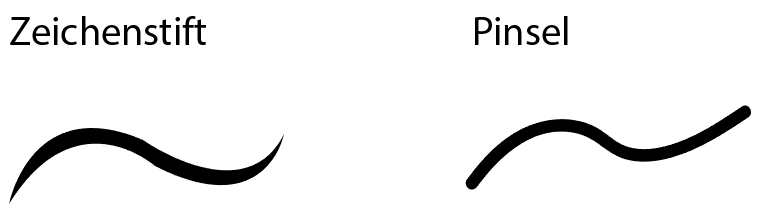
\includegraphics[width=0.7\textwidth]{design_abb2.png}
  \caption{Vergleich von Zeichenstift und Pinsel}
\end{figure}

\paragraph{Das Ellipse-Werkzeug}
\leavevmode \\
Für die runden Elemente, wie Iris, Pupille und die Reflexionen, wurde das Ellipse-Werkzeug verwendet. Ellipsen benötigen nur drei Parameter um als Vektorgrafik beschrieben zu werden. Der Ursprungspunkt, welcher die linke obere Ecke ist, die Höhe und die Breite. Es gibt zwei verschiedene Möglichkeiten das Ellipse-Werkzeug zu verwenden. Man kann mit dem Cursor auf den Ursprungspunkt klicken, die Maus gedrückt halten und dann die Ellipse auf die gewünschte Höhe, beziehungsweise Breite ziehen. Wenn man bei diesem Prozess die Shift-Taste gedrückt hält, bleibt die Höhe und Breite gleich und man zeichnet somit einen perfekten Kreis. Eine andere Möglichkeit ist es, mit dem Ellipse-Werkzeug in den Ursprungspunkt der Ellipse zu klicken. Daraufhin öffnet sich ein Fenster, bei dem man Höhe und Breite manuell angeben kann. Für einen Kreis nimmt man einfach zwei idente Werte, wie zum Beispiel 100 Pixel Höhe und 100 Pixel Breite.\footnote{\label{} vgl.https://helpx.adobe.com/at/illustrator/using/drawing-simple-lines-shapes.html\#draw\_ellipses [Zugriff: 26.03.2018]}
\leavevmode \\

\paragraph{Pathfinder}
\leavevmode \\
Um dem Auge mehr persönlichen Charakter und Dynamik zu geben, wurde die Kreisform, der Iris auf der oberen Seite etwas abgeflacht. Um dieses Ergebnis zu erlangen wurde ein flacher Teil, des Kreises abgeschnitten. Bewerkstelligt, wurde dies durch Pathfinder-Effekte. Bei den Pathfinder-Effekten handelt es sich im Prinzip um die Kombination mehrerer Objekte, durch verschiedenste Interaktionsmodi. Die Interaktion selbst kann vom User jedoch nicht selbst bearbeitet werden. Es folgen nun vier Beispiele für solche Modi, darunter der, der für das Logo verwendet wurde.\footnote{\label{} vgl.https://helpx.adobe.com/de/illustrator/using/combining-objects.html [Zugriff: 27.03.2018]}
\footnote{\label{} vgl.https://helpx.adobe.com/de/illustrator/using/combining-objects.html\#pathfinder  [Zugriff: 27.03.2018]}
\leavevmode \\
\leavevmode \\
Hinzufügen:
\leavevmode \\
Dieser Modus zeichnet die die Kontur aller ausgewählten Objekte nach, um so die Kontur eines Ganzen zu erhalten.
\leavevmode \\
\leavevmode \\
Schnittmenge bilden:
\leavevmode \\
Zeichnet die Kontur des Bereiches nach, der von allen ausgewählten Objekten überlappt wird.
\leavevmode \\
\leavevmode \\
Subtrahieren:
\leavevmode \\
Das vordere Objekt wird vom hinteren Objekt abgezogen. Dieser Modus wäre für das Abschneiden der oberen Iris optimal gewesen, wurde aber nicht verwendet.
\leavevmode \\
\leavevmode \\
Unterteilen:
\leavevmode \\
Dieser Modus wurde für das Logo verwendet. Er teilt alle ausgewählten Objekte in eigene Teilflächen auf. Eine Teilfläche ist somit ein Bereich, der von keiner Linie, oder keinem Liniensegment unterteilt wird. Somit wurde im Falle, des Logos ein neues Objekt erstellt, welches das Segment, der Iris abdeckte, welches entfernt werden sollte. Nach Anwendung des Unterteilen-Modus entstanden drei verschiedene Flächen. Die abgeflachte Iris, der Schnittpunkt, der vollen Iris mit dem neuen Objekt und als letztes ein kleiner Teil, des neuen Objektes, der nicht in der Schnittmenge lag. Am Schluss mussten nur noch die zwei überflüssigen Objekte entfernt werden. Die Prozedur war somit umständlicher, als einfach den Subtrahieren-Modus anzuwenden.
\leavevmode \\

\paragraph{Glätten-Werkzeug}
\leavevmode \\
Die Augenbraue und die zwei anderen schwungvollen Striche, die die Konturen des Auges andeuten sollen, waren nicht sehr glatt. An einigen Stellen haben sich kleine Dellen oder Kanten gebildet, wenn zum Beispiel zwei aneinander liegende Kurven des Pfades sich nicht optimal ergänzt haben. Auch der Kreis, der die Iris bildet hatte an der abgeschnittenen Stelle ein sehr kantiges Aussehen, welche das Gesamtbild, dass aus vielen Rundungen besteht, aus der Ruhe brachte. Die einfachste und gleichzeitig zielführendste Methode war es, das Glätten-Werkzeug zu verwenden. Mit diesem Werkzeug kann man entlang eines Pfades, oder auch Pfadsegments fahren, um dieses zu glätten. Man kann das gezielte Segment auch mit dem Werkzeug vereinfachen, indem die Anzahl der Ankerpunkte reduziert wird. Dies passiert automatisch im Laufe, des Glättungsprozesses. Weniger Ankerpunkte bedeuten eine kleinere Datei. Wie bei den meisten Werkzeugen im Illustrator, ist es auch noch möglich den Toleranzbereich, des Tools und die Stärke, beziehungsweise die Effektivität einzustellen.\footnote{\label{} vgl.https://helpx.adobe.com/at/illustrator/using/editing-paths.html  [Zugriff: 27.03.2018]}

\begin{figure}[H] 
  \centering
     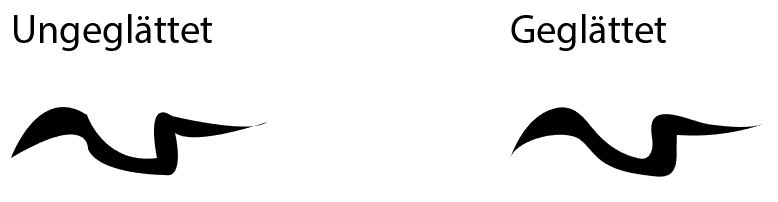
\includegraphics[width=0.7\textwidth]{design_abb3.png}
  \caption{Auswirkungen des Glätten-Werkzeuges}
\end{figure}

\paragraph{Farbe}
\footnote{\label{} vgl.https://helpx.adobe.com/at/illustrator/using/painting-fills-strokes.html [Zugriff: 28.03.2018]}
\leavevmode \\
Nachdem die Form des Logos schön rund und stimmig war, musste es noch eingefärbt werden. Hierbei war es wichtig zu wissen, dass es Konturen und Flächen gibt.
\leavevmode \\
\leavevmode \\
Flächen:
\leavevmode \\
Eine Fläche ist grundsätzlich eine Farbe. Sie kann aber auch ein Farbverlauf oder ein Muster sein. Dies Fläche kann auf Objekte jeder Art angewandt werden, also ist es egal, ob das Objekt offen oder geschlossen ist. Außerdem kann man sie auch bei Teilflächen interaktiver Malgruppen verwenden.
\leavevmode \\
\leavevmode \\
Konturen:
\leavevmode \\
Bei einer Kontur handelt es sich um den Umriss eines Objektes. Dabei muss beachtet werden, dass es sich dabei nur um den sichtbaren Umriss handelt. Offene Objekte werden nicht komplett von Konturen umschlossen, sondern nur zum Teil. Eine Kontur kann auch der Pfad, oder die Kante einer interaktiven Malgruppe sein. Genau wie bei der Fläche, kann man auch hier Farben bestimmen, jedoch über die Möglichkeiten, der Fläche hinaus, kann man mit Hilfe der Pfadoptionen ob die Kontur beispielsweise gestrichelt sein soll. Eine weitere Option für Konturen, ist es ihre Stärke einzustellen. Man muss dabei aber beachten, dass diese nicht dynamisch ist. Wenn man zum Beispiel alle Pfade einer Grafik markiert, um sie zu verkleinern, hat die Kontur immer noch die selbe Stärke und wirkt dadurch dann viel dicker als zuvor. Ihre Stärke muss dann, der Größe entsprechend manuell angepasst werden.

\begin{figure}[H] 
  \centering
     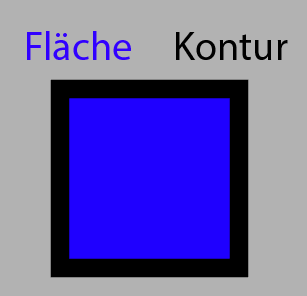
\includegraphics[width=0.4\textwidth]{design_abb4.png}
  \caption{Veranschaulichung von Fläche/Kontur}
\end{figure}

\leavevmode \\
\leavevmode \\
Also kann jedes Objekt mit einer Fläche und Kontur versehen werden. Es ist aber natürlich auch möglich nur eines der beiden, oder gar nichts auszuwählen, wobei letzteres in kaum einem Fall Sinn macht, da das Objekt dann komplett unsichtbar wäre. Zur einfachen Bedienung gibt es zwei Schaltflächen im Illustrator. Ein ausgefülltes Quadrat und die ausgefüllte Kontur eines Quadrats. Ein Doppelklick auf eines der beiden Elemente öffnet ein neues Fenster mit einem Farbwähler. Hier kann man mit Hilfe eines Schiebereglers und einer Art Koordinatensystem gewünschte Farben aussuchen. Genauer und somit auch zielführender, kann man die Farbwerte nach dem RGB-Modell, dem HSB-Modell, dem CMYK-Modell und hexadezimal angeben\footnote{\label{} vgl.https://helpx.adobe.com/de/illustrator/using/selecting-colors.html [Zugriff: 28.03.2018]}.
\leavevmode \\
\leavevmode \\
RGB:
\leavevmode \\
Bei dem RGB-Modell setzen sich die Farben aus den drei Grundfarben Rot, Grün und Blau zusammen. Daher auch der Name. Die einzelnen Anteile sind von bis zu einem Wert von 255 definierbar. Mit Null mitgezählt macht das also 256 verschiedene Stufen, also entspricht das acht Bit pro Grundfarbe. Die Reihenfolge bei RGB ist wichtig. So steht der erste Wert für Rot, der zweite für Grün und der letzte für Blau. Zum Beispiel hat man mit den Werten 255/0/0 ein reines Rot mit einem Rotanteil von 100\%.\footnote{\label{} vgl.http://www.webmasterpro.de/design/article/das-rgb-farbsysteme.html [Zugriff: 28.03.2018]}
\leavevmode \\
\leavevmode \\
HSB:
\leavevmode \\
Dieses Farbraumsystem beschreibt nicht durch Farbmischungen von Grundfarben, sondern durch die Eigenschaften, der Farben. H steht für das englische Wort „hue“ und gibt den Farbton als Farbwinkel an. Also kann der Farbton von Null bis 360 Grad angegeben werden. S steht für „saturation“, also die Sättigung der Farbe. Diese beschreibt den Grauanteil der Farbe. Das heißt, dass ein Wert von null Prozent ein Grau ergeben würde und ein Wert von 100 Prozent einen voll gesättigten Farbton. B wird auch in Prozent angegeben uns steht für „brightness“, also Helligkeit.\footnote{\label{} vgl.http://www.webmasterpro.de/design/article/farblehre-uebersicht-farbraeume.html [Zugriff: 28.03.2018]}
\footnote{\label{} vgl.http://www.win-seminar.de/adobe/hsb-farbmodell.php [Zugriff: 28.03.2018]}
\leavevmode \\
\leavevmode \\
CMYK:
\leavevmode \\
Hier stehen die Buchstaben für Cyan, Magenta, Yellow und Key. Cyan ist ein helles Blau mit grünlichem Ton. Bei Magenta handelt es sich um ein leicht violett getöntes Rot. Yellow ist ein helles strahlendes Gelb. Key ist einfach schwarz. Die Mischung aus Cyan, Magenta und Yellow würde zwar auch Schwarz ergeben, jedoch ist Key ein weiterer Parameter von CMYK, da das Schwarz aus den drei anderen Farben nicht besonders intensiv oder rein ist. Die Farbanteile, der einzelnen Farben werden in Prozent angegeben. CMYK hat im Vergleich zu RGB einen sehr kleinen Farbraum. Somit kann man nicht das selbe Farbspektrum veranschaulichen. Es ist aber gut geeignet um Objekte zu designen, die im Anschluss gedruckt werden sollen, da Drucker nicht das komplette RGB-Spektrum abdecken können. Je nachdem ob man mit RGB oder CMYK arbeitet, ist es empfehlenswert, den Dokumentfarbmodus im Illustrator entsprechen anzupassen.\footnote{\label{} vgl.http://www.webmasterpro.de/design/article/das-cmyk-farbmodell.html [Zugriff: 28.03.2018]}
\leavevmode \\
\leavevmode \\
Hexadezimal:
\leavevmode \\
Hexadezimal ist im Prinzip eine andere Schreibweise für die RGB-Werte. Der Code besteht aus einem \# und daraufhin folgend sechs Zeichen. Diese können Null bis Neun und A bis F sein. Die ersten zwei Zeichen stehen für Rot, die zweiten für Grün und die dritten für Blau. Das bedeutet 256 verschiedene Möglichkeiten und acht Bit pro Farbe, also genau dieselben Werte, wie sie schon bei RGB zu lesen sind.\footnote{\label{} vgl.http://www.farbtipps.de/farben-digital/websichere-farben.html [Zugriff: 28.03.2018]}
\leavevmode \\
\leavevmode \\
Websichere Farben:
\leavevmode \\
In dem Farbwahlfenster gibt es außerdem die Möglichkeit, nur websichere Farben auswählbar zu machen. Das kann sehr hilfreich sein, da nicht jeder Browser alle Farben unterstützt. Wenn man websichere Farben nutzt, kann man sich als Designer sicher sein, dass jeder Nutzer genau die selben Farben sieht. Eine websichere Farbe hat im Hexadezimalcode an jeweils der Rot-, Grün- und Blaustelle die Zeichenkombinationen 00, 33, 66, 99, CC oder FF stehen. Das heißt aber, dass es nur 216 verschiedene Farben gibt, die als websicher gelten.\footnote{\label{} vgl.http://www.farbtipps.de/farben-digital/websichere-farben.html [Zugriff: 28.03.2018]}
\leavevmode \\
\leavevmode \\
Wenn man nun eine Farbe für jeweils Fläche und Kontur festgelegt hat, kann man diese mit der Schaltfläche „Fläche und Kontur vertauschen“ einfach austauschen.
\leavevmode \\
\leavevmode \\
Füllarten:
\leavevmode \\
Unter der Fläche- und Konturschaltfläche befinden sich drei weitere kleinere. Die erste, ist die bisher beschriebene „Farbe“. Wenn man sie auswählt, wird die derzeitig ausgewählte Farbe auf die Fläche oder Kontur angewandt. Bei dem Logo wurde Farbe bei den Flächen, der schwarzen Linien, der Pupille, der Reflexion und der Kontur, der Iris verwendet.
\leavevmode \\
Die zweite Schaltfläche ist der „Verlauf“. Mit ihr kann man Farbverläufe auf Flächen und Konturen anwenden. Es bieten sich neben den bereits erläuterten Farbwahloptionen auch die Möglichkeiten zu entscheiden, welche und wie viele Farben der Verlauf in welcher Reihenfolge abdecken soll, ob der Verlauf linear oder kreisförmig sein soll und welchen Winkel der Verlauf haben soll. Außerdem gibt es drei verschiedene Einstellungsmöglichkeiten, wie der Verlauf auf Konturen angewendet werden soll. Die Fläche, der Iris wurde mit einem Verlauf versehen. Dieser verläuft gleichmäßig und linear von Orange zu Grün, wobei Orange linksseitig und Grün rechtsseitig ist.
\leavevmode \\
Bei der dritten Schaltfläche, „Ohne“, handelt es sich um die einfache Option, die Fläche oder Kontur leer zu lassen. Das bedeutet, wenn man beispielsweise bei einem Objekt eine schwarze Kontur ohne Fläche hat, ist die Fläche innerhalb der Kontur transparent und weiter hinten liegende Objekte sind dadurch sichtbar. Bei dem Logo wurde jedoch kein „Ohne“ verwendet.\footnote{\label{} vgl.https://helpx.adobe.com/at/illustrator/using/painting-fills-strokes.html [Zugriff: 28.03.2018]}

\paragraph{Textwerkzeug}\footnote{\label{} vgl.https://helpx.adobe.com/at/illustrator/using/creating-text.html [Zugriff: 29.03.2018]}
\leavevmode \\
Zuletzt wurde bei dem Logo noch der Schriftzug „Insight“ angefügt. Dafür muss man einfach nur das Text-Werkzeug auswählen und damit an die Stelle klicken, an der der Text beginnen soll. Dieser kann dann einfach geschrieben werden. In den Texteinstellungen kann man noch Eigenschaften, wie Textgröße, Font und Zeilenabstand angeben\footnote{\label{} vgl.https://helpx.adobe.com/at/illustrator/using/fonts.html [Zugriff: 29.03.2018]}.
Für den Schriftzug, des Logos wurde Parisien Night Oblique als Font gewählt. Diese Schrift wurde wegen des Logos in das Corporate Design aufgenommen. Die schwungvolle dynamische Linienführung soll an die Eigenschaften, des Logos erinnern. Zusammen ergeben Signet und Schriftzug ein stimmiges Bild, was zeigt, dass die Wahl, der richtigen Font für ein Logo ein essenzieller Faktor ist. Näheres zur Typografie, ist beim Corporate Design zu lesen.
\leavevmode \\
\leavevmode \\
Verformen mit Hüllen:
\leavevmode \\
Die Schrift sollte sich an das Logo schmiegen, welches eine sehr runde Erscheinungsform hat. Deshalb musste die Schrift gekrümmt und rotiert werden. Bei der Rotation handelte es sich um eine einfache Transformation des Objekts, welche mit dem Cursor, oder manuell mit der Angabe von Winkelgrad umgesetzt werden konnte. Um die Schrift jedoch entlang der Linien zu krümmen, wurden Hüllen verwendet. Bei Hüllen handelt es sich Objekte, die verwendet werden um ausgewählte Objekte zu verformen. Dafür findet man unter der Schaltfläche „Objekt“ die Kategorie „Verzerrungshülle“. Die erste Option, „Mit Verkrümmung erstellen…“, ist gleich die, die benötigt wurde. Es öffnet sich ein neues Fenster, in welchem man die Art der Verkrümmung angeben kann. Im Fall des Schriftzuges ist diese Art „Bogen“. Um nun den Anfang und das Ende, des Textes nach oben zu biegen, um ihn an das Logo anzupassen, muss nur noch ein negativer Prozentwert angegeben werden. Minus 20 Prozent erwiesen sich als eine sehr leichte, aber doch passende Krümmung.\footnote{\label{} vgl.https://helpx.adobe.com/at/illustrator/using/reshape-using-envelopes.html [Zugriff: 29.03.2018]}
\leavevmode \\
\leavevmode \\
SVG:
\leavevmode \\
Nachdem es fertiggestellt wurde, wurde das Logo, so wie fast alle anderen im Illustrator erstellten Grafiken, als SVG abgespeichert. Hierbei handelt es sich um ein auf XML basierendes Dateiformat, welches genutzt wird um Vektorgrafiken im Web darzustellen.\footnote{\label{} vgl.https://liechtenecker.at/svg-die-zukunft-von-grafiken-auf-webseiten/ [Zugriff: 29.03.2018]}

\begin{figure}[H] 
  \centering
     
\includegraphics[width=0.4\textwidth]{design_abb5.png}
  \caption{Logo Endergebnis}
\end{figure}

\subsection{Visitenkarten}
\subsubsection{Zweck}
Die Visitenkarten von Insight wurden für den Tag der offenen Tür und den Innovation Day an der HTL Rennweg gedruckt. Ihr Zweck war es, Besucher, der Schule und Unternehmen auf das Projekt aufmerksam zu machen und ihnen die Möglichkeit zu geben, später Informationen zu dem Projekt zu finden, oder Kontakt zu dem Team aufzunehmen.
\subsubsection{Umsetzung}

\paragraph{Neue Datei}
\leavevmode \\
Auch die Visitenkarte wurde im Adobe Illustrator entworfen. Das erste worauf geachtet werden musste ist, dass die Datei die richtige Größe hat. Die ausgewählte Druckerei verlangte für jeweils die Vorder- und Rückseite, der Visitenkarte ein JPG, welches 85 Millimeter breit ist und 55 Millimeter hoch. Der Illustrator bietet bei der Erstellung, der Datei die Option Höhe und Breite in Millimetern anzugeben, was dem Entwurf der Karte sehr zu Gunsten kam. Der eingestellte Farbraum in den Dokumenteinstellungen war in diesem Fall CMYK, da dies für den anschließenden Druck optimal war. Außerdem wurde es von der Druckerei empfohlen, diesen Farbraum zu nutzen.\footnote{\label{} vgl.https://helpx.adobe.com/at/illustrator/how-to/create-new-document.html [Zugriff: 30.03.2018]}

\paragraph{Vorderseite}
\leavevmode \\
Auf der Vorderseite sollten alle wichtigen Informationen stehen, welche geplant waren auf der Visitenkarte preis zu geben. Dazu gehört das Logo, die URL der Website, die Mailadresse, des Teams und der Name, der Schule. Der Name, des Projekts konnte außenvor gelassen werden, da er sich bereits im Logo befindet. So wurde überflüssiger Content vermieden und das Gesamtbild aufgeräumter gehalten. Das Layout ist zentriert und die Elemente untereinander angeordnet. Das Schmalste ganz oben und das Breiteste unten. So erscheint der Content der Vorderseite wie ein Dreieck oder Pyramide, also ein Objekt womit der Betrachter vertraut ist. In einem, nach Corporate Design, orangenen Footer, ist optisch abgegrenzt von den restlichen Inhalten, der Name, der Schule.
\leavevmode \\
\leavevmode \\
Intelligente Hilfslinien: 
\leavevmode \\
Zur Positionierung, der Elemente auf der Karte, wurden intelligente Hilfslinien verwendet. Diese lassen Ankerpunkte von Objekten, anhand von Ankerpunkten anderer Objekte relativ positionieren. Das heißt, wenn diese Hilfslinien aktiviert sind, lassen sich Objekte so positionieren, dass sie zum Beispiel mittig von einem anderen Objekt liegen, oder an einer markanten Stelle vertikal, oder horizontal gleich mit einer markanten Stelle des Anderen Objektes liegen. So wurden alle Elemente perfekt mittig untereinander platziert. Die selbe Technik wurde beim Logo verwendet, um die Pupille in der Mitte, der Iris zu platzieren. Für die Schrift wurde das Textwerkzeug verwendet. Um das Logo auf die Karte zu übertragen, wurden die Pfade kopiert und eingefügt. Beim Verkleinern auf eine angemessene Größe, fiel die statische Stärke, der Kontur, der Iris auf. Diese musste manuell verringert werden, damit das Gesamtbild dem Original entsprach.\footnote{\label{} vgl.https://helpx.adobe.com/de/illustrator/using/rulers-grids-guides-crop-marks.html [Zugriff: 30.03.2018]}

\begin{figure}[H] 
  \centering
     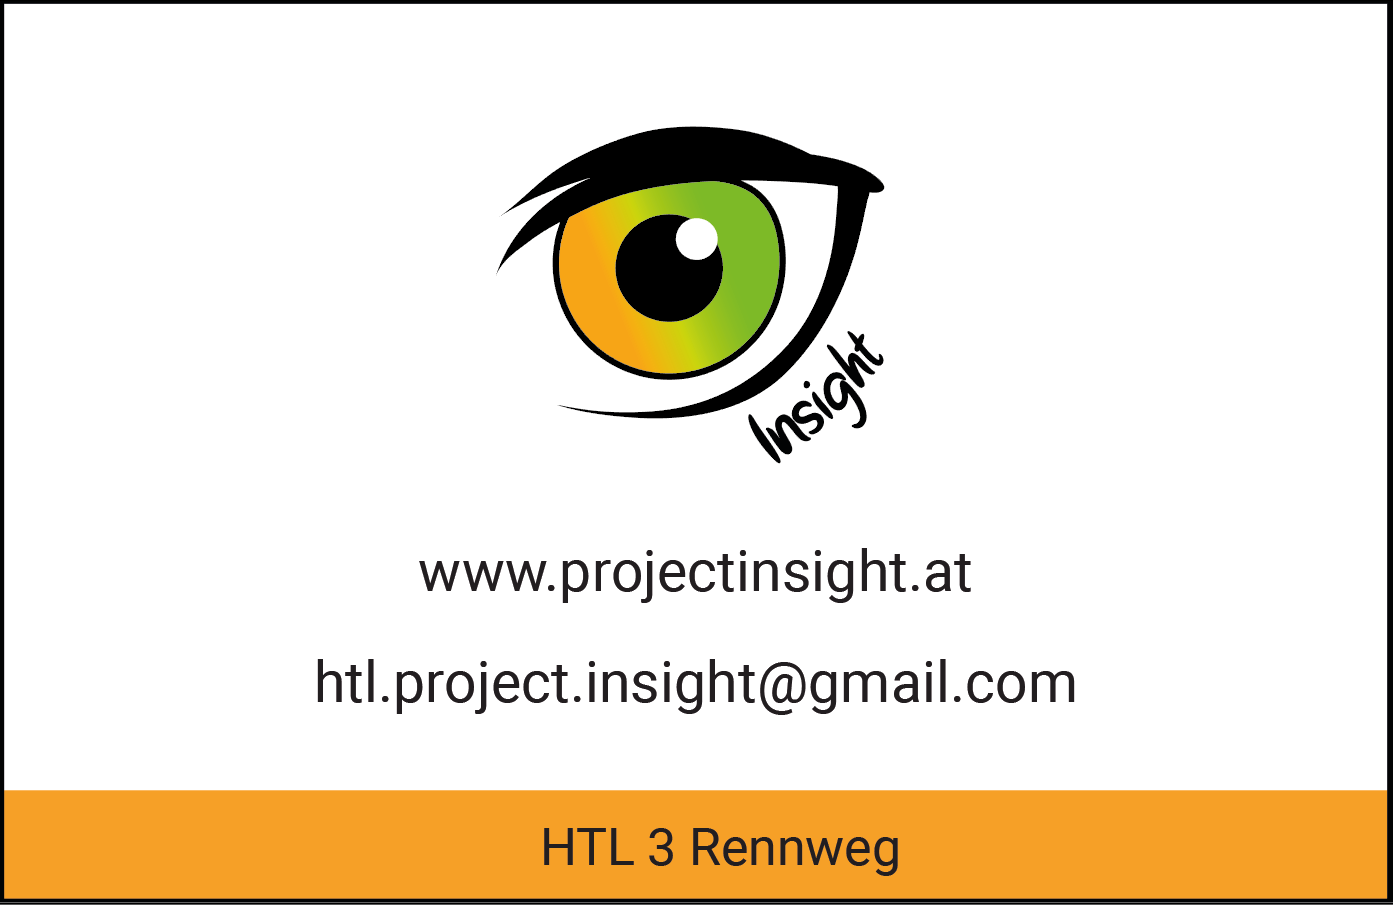
\includegraphics[width=0.5\textwidth]{design_abb6.png}
  \caption{Vorderseite der Visitenkarte}
\end{figure}

\paragraph{Rückseite}
\leavevmode \\
Auf der Rückseite der Visitenkarte prangt eine großer, mit Hilfslinien zentrierter, orange-grüner QR-Code, der den Scannenden auf die Website von Insight bringt. Der Code wurde per Eingabe, der URL in einem Online-Tool generiert und gedownloadet\footnote{\label{} http://goqr.me/de/\#t=url [Zugriff: 30.03.2018]}. Das erhaltene PNG wurde dann im Photoshop mit den Farben, des Corporate Designs eingefärbt.
\leavevmode \\
\leavevmode \\
QR-Code:  
\leavevmode \\
QR steht für „Quick Response“. Bei dem Code handelt es sich um eine quadratische Matrix aus kleineren weißen und schwarzen Quadraten. Die Codes können mit Hilfe einer App, von Handykameras gelesen werden und so Informationen oder Daten ausgeben. Im Fall der Visitenkarte, handelt es sich um eine URL. Damit der Code funktioniert, egal wie er gedreht ist, befinden sich in drei von vier Ecken der Matrix, größere Quadrate. An ihnen wird sich am Scanvorgang orientiert, wie herum der Code korrekt zu lesen ist.\footnote{\label{} vgl.http://www.t-online.de/digital/smartphone/id\_46404754/was-sind-qr-codes-und-wie-nutzt-man-sie-.html [Zugriff: 30.03.2018]}

\begin{figure}[H] 
  \centering
     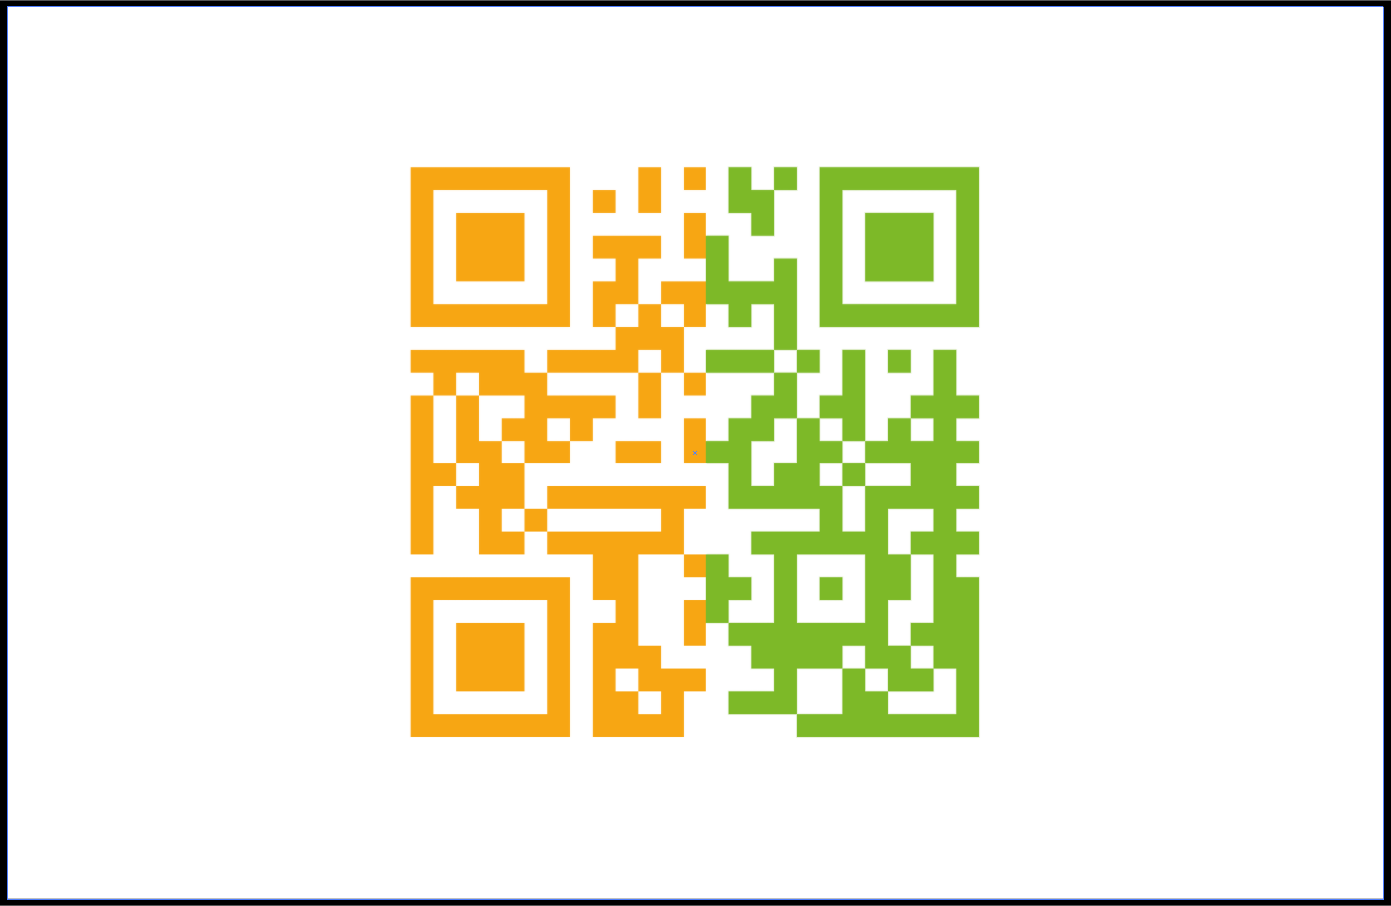
\includegraphics[width=0.5\textwidth]{design_abb7.png}
  \caption{Rückseite der Visitenkarte}
\end{figure}

\subsection{Designelemente}
\subsubsection{Zweck}
Mit Designelementen sind weitere selbst erstellte Grafiken gemeint, die auf der Webseite Verwendung gefunden haben. Manche dieser Grafiken wurden auf Grund von Änderungen nicht in die finale Version der Website aufgenommen. Die folgenden Grafiken sind Teil, der finalen Version und als Userinteraktives Element implementiert.
\leavevmode \\
\leavevmode \\
Schrödingers Katze:
\leavevmode \\
Die Katze in der Box wurde wie das Logo zuerst im Photoshop skizziert und dann im Illustrator mit dem Zeichenstift-Werkzeug nachgezeichnet. Im Gegensatz zu den bisher erwähnten Grafiken, wurden die Kopier- und Einfügeoption viel öfter verwendet. Um Objekte zu kopieren, muss man sie einfach nur auswählen und die Tastenkombination „Strg“ + „C“ verwenden. Um ein Objekt einzufügen nutzt man „Strg“ + „V“. Die Funktion wurde bei der geschlossenen Box für die Schrauben und diverse Planken genutzt, damit sie exakt die selbe Größe haben. Bei der offenen Box wurde Kopieren und Einfügen wiederum für das Holz benutz, aber diesmal auch für die Maserung, die Augen und Pfoten, der Katze und sogar ihrem Mund. Verwendet wurde Katze im Chapter 7 der Website. Das Spiel heißt Schrödingers Katze.\footnote{\label{} vgl.http://pixus-punktus.de/kopieren-und-einfuegen-in-illustrator [Zugriff: 30.03.2018]}

\begin{figure}[H] 
  \centering
     
\includegraphics[width=0.4\textwidth]{design_abb8.png}
  \caption{Katze Endergebnis}
\end{figure}

\leavevmode \\
\leavevmode \\
Rakete: 
\leavevmode \\
Auch die Rakete wurde mit dem Zeichenstift-Werkzeug erstellt. Jedoch nur die Hälfte. Um die Rakete symmetrisch zu machen, wurde nur die Hälfte gezeichnet, dann durch Kopieren und Einfügen dupliziert und anschließend wurde die kopierte Hälfte gespiegelt und an die zweite Hälfte angefügt. Gespiegelt wurde das Objekt mit dem Spiegeln-Werkzeug. Mit Hilfe der Shift-Taste konnte man den Spiegel-Winkel auf 45-Grad-Schritte beschränken, was ein gespiegeltes Gegenstück erzeugte, welches perfekt an sein Ursprungsobjekt anschloss. Die Rakete war ursprünglich als Button auf der Website geplant, hat aber nun als Userinteraktives Element bei „Verschiebe das Universum“ seinen Platz gefunden.\footnote{\label{} vgl.https://helpx.adobe.com/de/illustrator/using/rotating-reflecting-objects.html [Zugriff: 30.03.2018]}

\begin{figure}[H] 
  \centering
     
\includegraphics[width=0.4\textwidth]{design_abb9.png}
  \caption{Rakete Endergebnis}
\end{figure}

\leavevmode \\
\leavevmode \\
Bezirkkarte von Wien:
\leavevmode \\
Es war ursprünglich geplant ein userinteraktives Element auf der Website einzubauen, welches eine Karte von Wien seien sollte. Je nachdem über welchem Bezirk man sich mit dem Cursor befand, sollte dieser eingefärbt werden. Dafür wurde eine farblose Karte benötigt und und jeweils eine Karte, wo jeweils ein Bezirk eingefärbt war. Die Karte war eine nervenzerreißende, lange Arbeit, da zu dem Zeitpunkt noch nicht an den Pathfinder gedacht wurde. Das heißt anstatt jeden Bezirk in ein eigenes, einfärbbares Objekt zu verwandeln, wurde für jeden Bezirk ein extra Objekt gezeichnet, welches eingefärbt werden konnte. Danach wurde für die leere Karte ein SVG abgespeichert und für jeden Bezirk zwei, da noch nicht feststand, ob die Bezirke Grün oder Orange sein sollten. Das Umfärben, Auswählen und und einzelne Abspeichern hat sehr viel Arbeitszeit in Anspruch genommen.

\begin{figure}[H] 
  \centering
     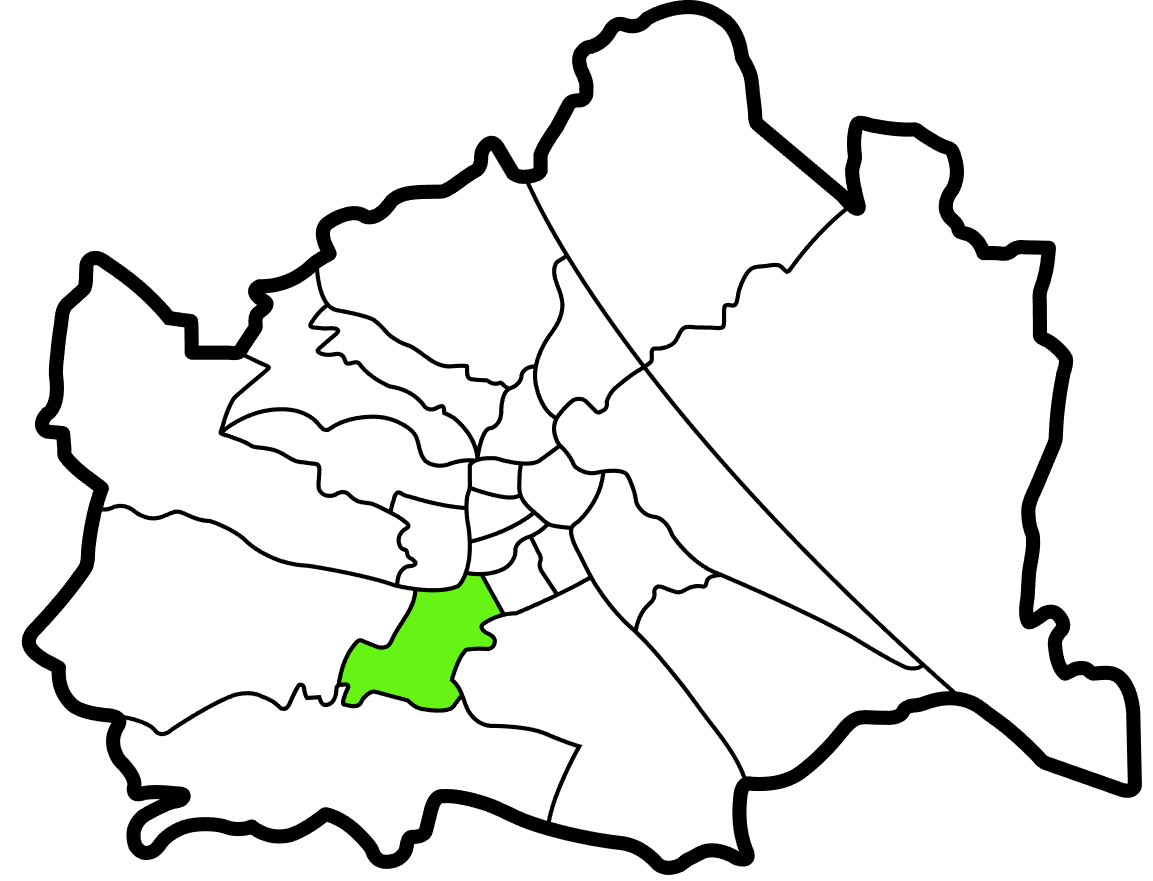
\includegraphics[width=0.4\textwidth]{design_abb10.png}
  \caption{Wienkarte Endergebnis}
\end{figure}